\documentclass[12pt]{article}
\usepackage{amsmath}
\usepackage{amssymb}
\usepackage{graphicx}
\usepackage{listings}
\usepackage{xcolor}
\usepackage{caption} % For better captions

% Define colors for code listings
\definecolor{codeblue}{rgb}{0.1, 0.1, 0.8}
\definecolor{codegray}{rgb}{0.5, 0.5, 0.5}
\definecolor{codepurple}{rgb}{0.58, 0, 0.82}
\definecolor{backcolour}{rgb}{0.95, 0.95, 0.92}

\lstdefinestyle{mystyle}{
    backgroundcolor=\color{backcolour},
    commentstyle=\color{codegray},
    keywordstyle=\color{codeblue},
    numberstyle=\tiny\color{codegray},
    stringstyle=\color{codepurple},
    basicstyle=\ttfamily\footnotesize,
    breakatwhitespace=false,
    breaklines=true,
    captionpos=b,
    keepspaces=true,
    numbers=left,
    numbersep=5pt,
    showspaces=false,
    showstringspaces=false,
    showtabs=false,
    tabsize=2
}

\lstset{style=mystyle}

\title{Longest Path Finder Using MapReduce}
\author{}
\date{}

\begin{document}

\maketitle

\section*{Introduction}
This report describes the implementation of a program that identifies the longest path(s) from a set of paths using a simplified MapReduce paradigm. The program reads paths from an input file, calculates their lengths, and identifies the longest path(s) efficiently.

\section*{Implementation Details}

\subsection*{Why This Implementation Was Chosen}
The program is implemented in C, leveraging its efficiency in handling memory and performing computational tasks. By structuring the program with Mapper and Reducer phases, the implementation aligns with the MapReduce approach, making the solution modular and easy to understand.

\subsection*{Mapper Functionality}
The Mapper phase reads paths from the input file and calculates their lengths. Each path and its length are stored in an array of structures. This step ensures that the data is prepared for further processing.

\begin{lstlisting}[language=C, caption=Mapper Phase]
char line[MAX_LINE_LENGTH];
while (fgets(line, sizeof(line), inputFile)) {
    line[strcspn(line, "\n")] = 0;  // Remove newline character

    if (pathCount < MAX_PATHS) {
        strcpy(pathLengths[pathCount].path, line);
        pathLengths[pathCount].length = strlen(line);
        pathCount++;
    } else {
        printf("Warning: Maximum number of paths exceeded. Some paths may be skipped.\n");
        break;
    }
}
\end{lstlisting}

\subsection*{Sorting Phase}
The paths are sorted by their lengths in descending order using the \texttt{qsort} function. This ensures that the longest path(s) are easily accessible for output.

\begin{lstlisting}[language=C, caption=Sorting Phase]
qsort(pathLengths, pathCount, sizeof(PathLength), comparePathLength);
\end{lstlisting}

\subsection*{Reducer Functionality}
The Reducer phase identifies the longest path(s) from the sorted array and writes them to the output file. All paths with the maximum length are included in the output.

\begin{lstlisting}[language=C, caption=Reducer Phase]
if (pathCount > 0) {
    int maxLength = pathLengths[0].length;
    for (int i = 0; i < pathCount; i++) {
        if (pathLengths[i].length == maxLength) {
            fprintf(finalOutputFile, "%s\n", pathLengths[i].path);
        }
    }
}
\end{lstlisting}

\section*{Program Workflow}

\begin{enumerate}
    \item The program reads paths from the input file.
    \item The Mapper calculates the lengths of each path and stores them in an array.
    \item The paths are sorted in descending order based on their lengths.
    \item The Reducer identifies and outputs the longest path(s).
\end{enumerate}

\section*{Figure}
The following figure illustrates the workflow of the program:

\begin{center}
    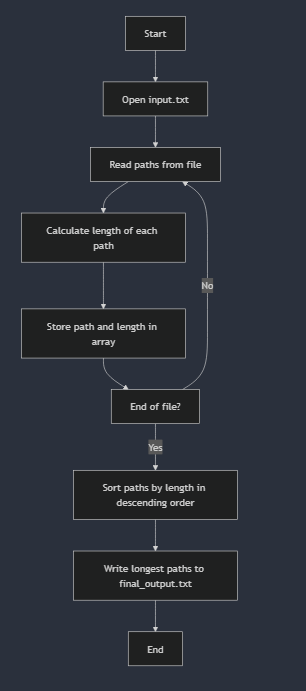
\includegraphics[width=0.8\textwidth]{lab5-flowchart.png} % Replace with actual diagram file
    \captionof{figure}{Mapper and Reducer Workflow for Longest Path Finder}
\end{center}

\section*{Conclusion}
This implementation efficiently identifies the longest path(s) from a set of input paths. By employing the MapReduce paradigm, the solution remains modular and extensible, making it suitable for similar problems involving path processing or length calculations.

\end{document}
